\documentclass{standalone}
\usepackage{pgfplots}
\usepackage[charter]{mathdesign}
\begin{document}
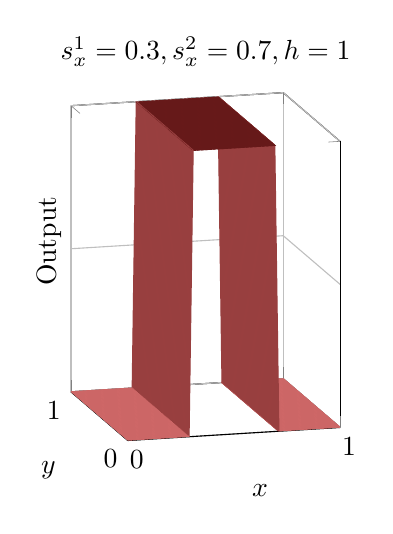
\begin{tikzpicture}[declare function = {step(\x,\s,\t) = 0.5*sign(\x-\s)-0.5*sign(\x-\t);}]
	\begin{axis}[colormap={justred}{rgb255=(255,127,127);rgb255=(127,31,31)},grid=major,width=5cm,height=6cm,view={-15}{10},xlabel={$x$},ylabel={$y$},zlabel={Output},title={$s^1_x=0.3,s^2_x=0.7, h=1$},zmin=0,zmax=1,xtick={0,1},ytick={0,1},zmajorticks=false]
		\addplot3[surf,domain=0:1, samples=53, shader=faceted]{
			1*step(x,0.3,0.7)};
	\end{axis}
\end{tikzpicture}
\end{document}
		